\subsection{Summary}

Let us summarize the procedure we use for approximating the solution of \eqref{eq:GeneralDarcySDE}. 
\begin{itemize}
	\item[--] Generate $A$ on a grid with spacing $\Delta_A$ with a Fourier transform method.
	\item[--] Approximate the solution of \eqref{eq:DarcyProblem} with the Finite Element methods on a fine triangulation $T_p$ with maximum element size $\Delta_p$.
	\item[--] Compute the velocity field from the FEM solution and interpolate it on a grid with spacing $\Delta_u$ to obtain a piece-wise constant field $\tilde{u}$.
	\item[--] Solve \eqref{eq:GeneralDarcySDE} with DEM or CEM to evaluate the mean exit time $\bar\tau$ using $\tilde{u}$ as the transport field.
\end{itemize}
Schematically, our procedure is the following
\begin{center}
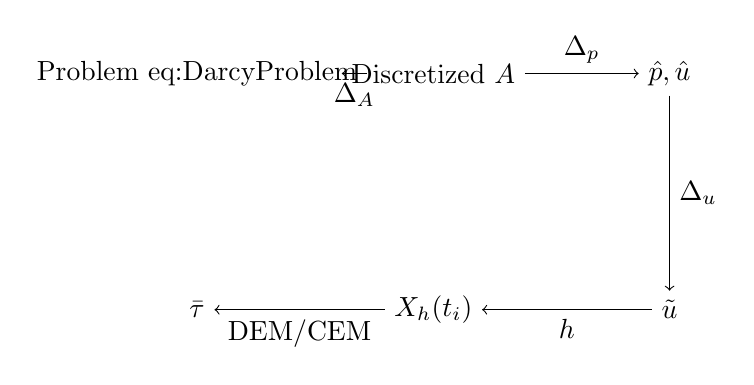
\begin{tikzpicture}[node distance=3cm, auto]
	\node (A) {Problem \eqref{eq:DarcyProblem}};
	\node (DPr) [right of=A]{Discretized $A$};
	\node (uh) [right of=DPr] {$\hat p, \hat u$};
	\node (Ux) [below of=uh] {$\tilde{u}$};
	\node (Xh) [left of=Ux] {$X_h(t_i)$};
	\node (tau) [left of=Xh] {$\bar\tau$};
  	
	\draw[->] (A) to node {$\Delta_A$} (DPr);
	\draw[->] (DPr) to node {$\Delta_p$} (uh);
	\draw[->] (uh) to node {$\Delta_u$} (Ux);
	\draw[->] (Ux) to node {$h$} (Xh);
	\draw[->] (Xh) to node {DEM/CEM} (tau);
\end{tikzpicture}
\end{center}
